\chapter{Background}
\label{cha:background}
\section{Constraint Satisfaction Problems}
A constraint satisfaction problem (CSP) consists of \cite{r18}:
\begin{itemize}
  \item a finite set of variables $V = \{{v_{1}, v_{2},..., v_{n}}\}$,
  \item a finite set of domains $D = \{D_{1}, D_{2},..., D_{n}\}$ such that for each
variable $v_{i} \in V$ there is a domain $D_{i}$ which is a finite set of objects that can be assigned to $v_{i}$,
  \item a finite set of constraints $C = \{C_{1}, C_{2},..., C_{k}\}$ such that the scope of each constraint is a subset of $V$. A constraint can be represented as a pair ($V_{s}$,$A_{s}$), where $V_{s}$ is a set of variables which is called scope and $A_{s}$ is a set of complete assignments for $V_{s}$.
\end{itemize}
"A solution to a \emph{CSP} is a complete instantiation of the variables in $V$ satisfying all the constraints in $C$"~\cite{r18}. Such a problem is usually solved by a form of search. However, it is an NP-complete problem which means that there does not exist an algorithm to solve it in polynomial time at the moment. Only if P=NP, there is such an algorithm. Therefore, solving a CSP in a reasonable time requires the combination of optimization methods. In our case, even though different solvers adopt various optimization methods (more details in Chapter 4), singleton arc consistency is commonly used by CSP solvers. "A variable $v$ is \emph{arc consistent} with respect to another variable $u$ if and only if for every $d \in D_{v}$ there is at least one $d'\in D_{u}$ such that $(d,d')\in C_{v,u}$"~\cite{r7}. Accordingly, a CSP is \emph{arc consistent} if and only if all pairs of variables are arc consistent with each other. Furthermore, "The value $a$ of the variable $v_{i}$ is \emph{singleton arc consistent} if and only if the problem restricted to $v_{i}=a$ (i.e., $D_{i}=\{a\})$ is arc consistent. The CSP is \emph{singleton arc consistent} if and only if every value of every variable is singleton arc consistent"~\cite{r30}.
Based on singleton arc consistency, the values that violate singleton arc consistency in the domains will be removed, which significantly decreases the number of search nodes so that it saves a lot of search time. Therefore, it takes up a vital position in the optimizations of CSPs. 
\section{Rotation Matrix}
Rotation matrices are used to perform rotations in Euclidean space. "\emph{Rotation} is the action of moving or causing to move in a circle round an axis or centre" and "\emph{Vector} is a quantity having direction as well as magnitude, especially as determining the position of one point in space relative to another" \cite{r14}. After the rotation of a vector, the magnitude which is the length of the vector will be preserved, only the direction of the vector will be changed. The process can be represented by a matrix operation such as 
\begin{equation}
V'=M.V,
\end{equation}
where $V$ is the input vector, $M$ is the rotation matrix and $V'$ is the output vector \cite{r15}. Therefore, the rotation matrices can be used to mathematically define rotations that can describe the placements for the pieces of the two games. In our case, the 2D rotation matrix will be used to model the puzzle game IQ twist and the 3D rotation matrix will be used to model the puzzle game Zig Zag Puzzler. For both games, only counter-clockwise rotations of 0, 90, 180 and 270 degrees will be considered for both the 2D Cartesian coordinate system which corresponds to x-axis and y-axis and the 3D Cartesian coordinate system which corresponds to the x-axis, y-axis, and z-axis.
\section{Minizinc Language}
Minizinc \cite{r10} is a simple and readily comprehensible constraint programming (CP) modelling language that intends to become the first standard modelling language for CP problems. The designers hope that Minizinc can be adopted by different solvers so that a modeller can compare different solvers for a problem. Minizinc usually appears together with the Minizinc-to-Flatzinc translator which transforms the Minizinc language into the Flatzinc language. Flatzinc \cite{r10} is a low-level solver-input language. Compared with Minizinc that is a high-level language, it is easier to be adapted by an interface, more effective and storage-saving but hard to understand for programmers. If a solver writer wants to support the Minizinc language, he or she just needs to write a simple Flatzinc front-end to their solver. As is shown in Figure 2.1, it plays the role of a bridge that connects the Minizinc file with respective interfaces for different solvers. 
\begin{figure}[htbp]
\centering
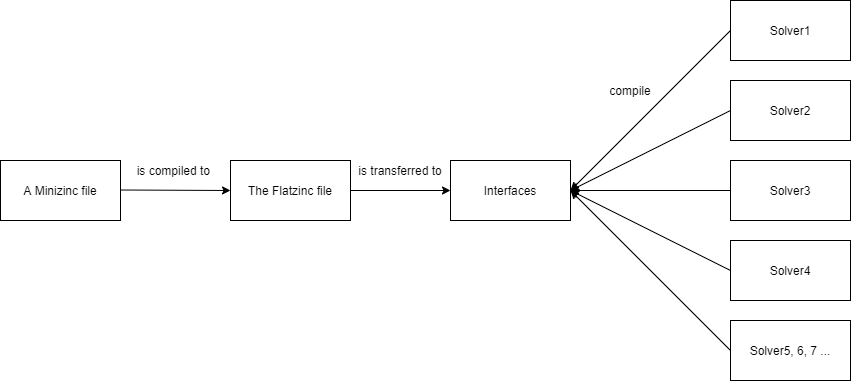
\includegraphics[width=0.8\linewidth]{figs/flowofMinizinc.png}
\caption{The process of a solver executing a Minizinc file}
  \label{fig:process}
\end{figure}
A Minizinc problem consists of two parts: the structure of the problem is corresponding to the model and the assignments to parameters for a particular problem are corresponding to the data. In addition, what it mainly supports has been listed below \cite{r10}:\\
\begin{compactenum}
  \item Scalar types: Booleans, integers and floats.
  \item Compound types: sets and arrays.
  \item Built-in operations: 
  \begin{compactitem}
  \item comparisons (e.g. <, ==),
  \item arithmetic operations (e.g. +, *, sum, min, mod, div),
  \item logical operations (e.g. $\vee$, $\wedge$, xor, forall),
  \item set operations (e.g. union, subset, in, card),
  \item array operations (e.g. length, index\_set),
  \item coercions (e.g. round, int2float, bool2int), 
  \item bounds operations (ub, lb, dom).
  \end{compactitem}
  \item Predicates: users can define their own predicates.
  \item Functions: users can define their own functions.
  \item Global constraints: 'globals.mzn' which includes all global constraints.
\end{compactenum}
In my case, the "$\vee$", "$\wedge$", "mod", "div", "alldifferent.mzn" from "globals.mzn", "set of int" and some functions have been used.
\begin{lstlisting}[language=minizinc,firstnumber=1]
% A simple Minizinc example 
include "alldifferent.mzn";% Equal to "globals.mzn"
\end{lstlisting}
The contents in line 1 are notes, which must start with a "\%". They provide explanations for the reader to understand the codes. And the contents in line 2 aim to call "alldifferent.mzn", which contains "alldifferent" constraint.
\begin{lstlisting}[language=minizinc,firstnumber=3]
%all the Vunits are different
constraint alldifferent([Vy11,Vy12,Vy13,Vy21,Vy22,Vy23,Vy24,Vy25,Vb11,Vb12,Vb13,Vb14,Vb15,Vb21,Vb22,Vb23,Vb24,Vg11,Vg12,Vg13,Vg14,Vg21,Vg22,Vg23,Vr11,Vr12,Vr13,Vr14,Vr21,Vr22,Vr23,Vr24]);
\end{lstlisting}
Accordingly, the contents in line 4 call the "alldifferent" constraint, which makes that there are no two variables equal to the same value. 
\begin{lstlisting}[language=minizinc,firstnumber=5]
set of int: position={
14,24,34,44,54,64,74,84,
13,23,33,43,53,63,73,83,
12,22,32,42,52,62,72,82,
11,21,31,41,51,61,71,81};
\end{lstlisting}
In line 5, the position has been defined, it is a set of int, and the numbers from line 6 to 9 represent the values in the set.
\begin{lstlisting}[language=minizinc,firstnumber=10]
var int:Vpr; var int:Vpb1;var int:Vpb2;var int:Vpg1;var int:Vpg2; var int:Vpy1;var int:Vpy2;
var position: Vb11;var position: Vb12;var position: Vb13;var position: Vb14;var position: Vb15;
\end{lstlisting}
From line 10 to 11, some variables and corresponding types have been defined. As an example, "var position: Vb11;" means Vb11 is a variable, and the type of Vb11 is "position". Therefore, the domain of Vb11 is the set of elements in position.
\begin{lstlisting}[language=minizinc,firstnumber=12]
function var int:g0(var int:a)=a mod 10;
function var int:g1(var int:a)=a div 10;
\end{lstlisting}
Moreover, from line 12 to line 13, the functions are defined by the user. The g0(a) will return the result of "a" mod 10, and g1(a) will return the result of "a" div 10.
\begin{lstlisting}[language=minizinc,firstnumber=14]
%blue piece2 
constraint (g0(Vb22) = g0(Vb21) + 1/\ g1(Vb22) = g1(Vb21)/\ g0(Vb23) = g0(Vb21) + 2/\ g1(Vb23) = g1(Vb21)/\ g0(Vb24) = g0(Vb21) + 3/\ g1(Vb24) = g1(Vb21)) \/
           (g0(Vb22) = g0(Vb21)/\ g1(Vb22) = g1(Vb21) + 1/\ g0(Vb23) = g0(Vb21)/\ g1(Vb23) = g1(Vb21) + 2/\ g0(Vb24) = g0(Vb21)/\ g1(Vb24) = g1(Vb21) + 3) \/
           (g0(Vb22) = g0(Vb21) - 1/\ g1(Vb22) = g1(Vb21)/\ g0(Vb23) = g0(Vb21) - 2/\ g1(Vb23) = g1(Vb21)/\ g0(Vb24) = g0(Vb21) - 3/\ g1(Vb24) = g1(Vb21)) \/
           (g0(Vb22) = g0(Vb21)/\ g1(Vb22) = g1(Vb21) - 1/\ g0(Vb23) = g0(Vb21)/\ g1(Vb23) = g1(Vb21) - 2/\ g0(Vb24) = g0(Vb21)/\ g1(Vb24) = g1(Vb21) - 3);
\end{lstlisting}
Accordingly, from line 15 to line 18, the functions have been used in the constraint. 
\\In addition, all codes above form part of the CSP model of IQ Twist.
